\documentclass[12pt]{article}

\usepackage[margin=1in]{geometry}
\usepackage{amsmath}
\usepackage{amssymb}
\usepackage{tikz}
\usetikzlibrary{arrows}
\usetikzlibrary{matrix}
\title{Linear Algebra Review}
\author{Arden Rasmussen}
\date{01 May 2017}
\linespread{1}
\begin{document}
\pagenumbering{gobble}
\maketitle
\newpage
\tableofcontents
\newpage
\pagenumbering{arabic}
\section{Abstract Vector Spaces/Dot-Product Spaces}\label{a}
\subsection{Abstract Vector Spaces}\label{a:a}
\begin{itemize}
  \item Set of $V$ called vectors
  \item Set of $Scalars$
  \item Vector Operators
  \begin{itemize}
    \item $\oplus$ Among vectors
    \item $\odot$ Between scalar and vector
  \end{itemize}
\end{itemize}
\subsubsection{$\oplus$}\label{a:a:p}
\begin{align}
  \left(\vec{v_1}\oplus\vec{v_2}\right)\oplus\vec{v_3} &= \vec{v_1}\oplus\left(\vec{v_2}\oplus\vec{v_3}\right)\\
  \text{There is some vector}\ \vec{0}\ &\text{with}\ \vec{v}\oplus\vec{0}=\vec{v}\ \text{for all}\ \vec{v}\\
  \text{For every}\ \vec{v}\ \text{there is some}\ \widetilde{\vec{v}}\ &\text{with}\ \vec{v}\oplus\widetilde{\vec{v}}=\vec{0}\\
  \vec{v_1}\oplus\vec{v_2}&=\vec{v_2}\oplus\vec{v_1}
\end{align}
\subsubsection{$\odot$}\label{a:a:d}
\begin{align}
  \left( \alpha + \beta \right) \odot \vec{v} &= \left( \alpha \odot \vec{v} \right) \oplus \left( \beta \odot \vec{v} \right)\\
  \alpha \odot \left( \vec{v_1} \oplus \vec{v_2} \right) &= \left( \alpha \odot \vec{v_1} \right) \oplus \left( \alpha \odot \vec{v_2} \right)\\
  \alpha \odot \left( \beta \odot \vec{v} \right) &= \left( \alpha \dot \beta \right) \odot \vec{v}\\
  1 \odot \vec{v} &= \vec{v}
\end{align}
\subsection{Sub-Space}\label{a:s}
\begin{itemize}
  \item $V$ is closed under $\oplus$:
    \begin{itemize}
      \item $\vec{v_1} \oplus \vec{v_2} \in V$
    \end{itemize}
  \item $V$ is closed under $\odot$:
    \begin{itemize}
      \item $\alpha \odot \vec{v} \in V$
    \end{itemize}
  \item $\oplus$ satisfies the axioms from~\ref{a:a:p} 
  \item $\odot$ satisfies the axioms from~\ref{a:a:d}
\end{itemize}
\subsection{Dot-Product Spaces}\label{a:d}
\begin{align}
  \left<\vec{x},\vec{x}\right> &\geq 0\\
  \left<\vec{x},\vec{x}\right> &= 0\ \text{If and only if}\ \vec{x} = \vec{0}\\
  \left<\vec{x},\vec{y}\right> &= \left<\vec{y},\vec{x}\right>\\
  \left<\alpha\vec{x} + \beta\vec{y},\vec{z}\right> &= \alpha\left<\vec{x},\vec{z}\right>+\beta\left<\vec{y},\vec{z}\right>
\end{align}
\subsection{Linear Transformation}\label{a:l}
\begin{itemize}
  \item $L(a+b) = L(a) + L(b)$
  \item $L(\alpha a) = \alpha L(a)$
\end{itemize}
\section{Linear (In) Dependence}
A set of vectors are linearly independent if the equation below holds true.
\begin{align}
  c_1\vec{v_1} + c_2\vec{v_2} + \cdots + c_n\vec{v_n} &= \vec{0}\\
  c_1=c_2=\cdots=c_n&=0
\end{align}
If the number of vectors is greater than the dimension, then the vectors are linearly dependent. To solve for linear independence use the following formula.
\begin{align}
  V &= \{\vec{v_1}, \vec{v_2}, \ldots, \vec{v_n}\}\\
  c_1\vec{v_1} + c_2\vec{v_2} + &\cdots + c_n\vec{v_n}\\
  \left( \begin{array}{ccccccc}
    v_1 & | & v_2 & | & \cdots & | & v_n
  \end{array}\right)\left(\begin{array}{c}
    c_1 \\ c_2 \\ \vdots \\ c_n
  \end{array}\right) &= \left(\begin{array}{c}
    0 \\ 0 \\ \vdots \\ 0
  \end{array}\right)
\end{align}
Finding the reduced row echelon form of the matrix of vectors will provide the answer. If the matrix is diagonal then the vectors are linearly independent, Otherwise one or more of the vectors can be written as a linear combination of the other vectors.
\par
Linear independence can also be found using the determinant of a matrix.
\begin{align}
  A_{n\times n}
  \det\left(A\right) &\neq 0\\
  \text{Then}\ &A^{-1}\ \text{exists}\\
  rref &= I\\
  Rank\left(A\right) &= n\\
  \text{Matrix is linearly independent}
\end{align}
\section{Basis/Coordinates/Dimension}\label{b}
\subsection{Basis}\label{b:b}
A basis is a set of vectors that span the entire space. And are linearly independent.
\begin{align}
  E &= \left[ \vec{e_1}, \vec{e_2}, \ldots, \vec{e_n} \right]\\
  Span\{E\} &= \text{Some space eg.}\ \mathbb{R}^3\\
  \text{Vectors of}\ &E\ \text{are linearly independent}
\end{align}
If the number of vectors in $E$ is equal to the dimension of the space, and the vectors of $E$ are linearly independent, then it is safe to assume that $E$ is a basis for that space.
\subsection{Coordinates}\label{b:c}
The coordinates of a vector can be found in terms of a linear combination of a basis. These coordinates can then be written as the coefficients of the basis vectors in the form of a vector in $\mathbb{R}^n$.
\begin{align}
  \vec{v} &= \alpha_1\vec{e_1} + \alpha_2\vec{e_2} + \cdots + \alpha_n\vec{e_n}\\
  {\left[\vec{v}\right]}_E &= \left(\begin{array}{c}
    \alpha_1 \\ \alpha_2 \\ \vdots \\ \alpha_n
  \end{array}\right)
\end{align}
This $\mathbb{R}^n$ vector can now be used in place of the initial vector, for other calculations.
\subsection{Dimension}\label{b:d}
Dimension is the measure of the number of ``Terms'' in a vector
\subsection{Change of Basis}\label{b:cb}
Changing basis fallows the diagram, where the matrix representation of a transformation can be represented with respect to any other basis.
\begin{figure}[h]
  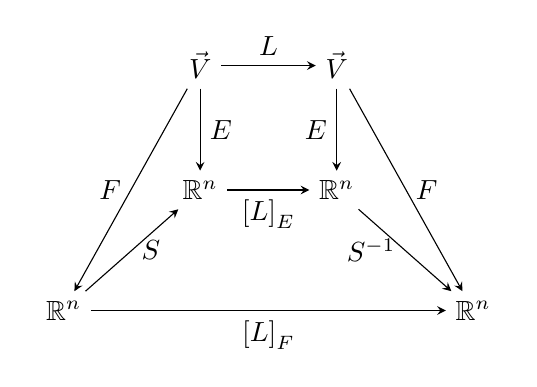
\begin{tikzpicture}
    \matrix(m)[matrix of math nodes, row sep=3em, column sep=3em]{
      \quad & \vec{V} & \vec{V} & \quad \\
      \quad & \mathbb{R}^n & \mathbb{R}^n & \quad \\
      \mathbb{R}^n & \quad & \quad & \mathbb{R}^n \\
    };
    \path[-stealth]
    (m-1-2) edge node[above]{$L$} (m-1-3)
    (m-1-2) edge node[left]{$F$} (m-3-1)
    (m-1-2) edge node[right]{$E$} (m-2-2)
    (m-1-3) edge node[right]{$F$} (m-3-4)
    (m-1-3) edge node[left]{$E$} (m-2-3)
    (m-2-2) edge node[below]{${\left[L\right]}_E$} (m-2-3)
    (m-3-1) edge node[right]{$S$} (m-2-2)
    (m-3-1) edge node[below]{${\left[L\right]}_F$} (m-3-4)
    (m-2-3) edge node[left]{$S^{-1}$} (m-3-4);
  \end{tikzpicture}
  \centering
\end{figure}
\begin{align}
  \vec{v} &= {E\left[\vec{v}\right]}_E\\
  \vec{v} &= {F\left[\vec{v}\right]}_F\\
  F &= ES\\
  {\left[\vec{v}\right]}_E &= S{\left[\vec{v}\right]}_F\\
  {\left[L\right]}_F &= S^{-1}{\left[L\right]}_ES\\
  {\left[L\right]}_E &= S{\left[L\right]}_FS^{-1}\\
  {\left[\vec{v}\right]}_E &= S{\left[\vec{v}\right]}_F
\end{align}
\section{Eigenstuff/Diagonalization}\label{e}
Eigenvalues ($\lambda$) and eigenvectors ($\vec{v}$) are vectors who's direction does not change during a transformation, but is stretched/flipped by a factor of the corresponding eigenvalue. This is ignoring the vector $\vec{v} = \vec{0}$, as that will always be true for these equations.
\begin{align}
  A\vec{v} &= \lambda\vec{v}\\
  A\dot \vec{v}-\lambda\vec{v} &= \vec{0}\\
  \left(A-\lambda I\right)\vec{v} &= \vec{0}
\end{align}
For a non-trivial $\vec{v}$ the matrix $\left(A -\lambda I\right)$ must have a $\det$ that equals $0$, because otherwise an inverse of that matrix exists, and the only $\vec{v}$ will be the trivial $\vec{0}$.
\begin{align}
  \det\left(A-\lambda I\right) &= 0\\
  \text{Solve for}\ &\lambda
\end{align}
In order to find eigenvectors from the eigenvalues, use rref on the matrix created by $\left(A - \lambda I\right)$, the resulting vector (s) will be the eigenvectors.
\section{Linear Transformations via Matrix Representation}\label{l}
First check that the transformation satisfies~\ref{a:l}. Then find the matrix representation of the transformation with respect to a basis.
\begin{align}
  L&:V\rightarrow V\\
  E &= \left[\vec{e_1},\vec{e_2},\ldots,\vec{e_n}\right]\\
  {\left[L\right]}_E &= \left(\begin{array}{ccccccc}
    {\left[L\left(\vec{e_1}\right)\right]}_E & | & {\left[L\left(\vec{e_2}\right)\right]}_E & | & \cdots & | & {\left[L\left(\vec{e_n}\right)\right]}_E
  \end{array}\right)
\end{align}
\section{Orthogonality/Dot-Product}\label{o}
\subsection{Dot-Product}\label{o:d}
Dot product functions must follow the axioms of a dot product~\ref{a:d}.
\begin{align}
  \Vert\vec{x}\Vert &= \sqrt{\left<\vec{x},\vec{x}\right>}\\
  \cos \gamma &= \frac{\left<\vec{x},\vec{y}\right>}{\Vert\vec{x}\Vert \cdot \Vert\vec{y}\Vert}\\
  \left<\vec{x},\vec{y}\right>=0 &\Rightarrow \vec{x} \perp \vec{y}
\end{align}
These rules of dot produce allow for some features.
\begin{align}
  -1 \leqq &\cos \gamma \leqq 1\\
  -1 \leqq &\frac{\left<\vec{x},\vec{y}\right>}{\Vert\vec{x}\Vert \cdot \Vert\vec{y}\Vert}\\
  -\Vert\vec{x}\Vert\dot\Vert\vec{y}\Vert \leqq &\left<\vec{x},\vec{y}\right> \leqq \Vert\vec{x}\Vert\cdot\Vert\vec{y}\Vert\\
  \Vert\vec{x}-\vec{y}\Vert &\leqq \Vert\vec{x}\Vert+\Vert\vec{y}\Vert
\end{align}
\subsection{Orthonormal-Basis}\label{o:o}
An orthogonal basis is a basis with all vectors that are orthogonal.
\begin{align}
  \left<\vec{e_i},\vec{e_j}\right> &= 0\\
  \text{For all}\ i\neq j
\end{align}
An orthonormal basis is a basis with orthogonal vectors, and normalized vectors.
\begin{align}
  \Vert\vec{e_i}\Vert &= 1\\
  \text{For all}\ i
\end{align}
A set of vectors $\vec{v_1},\vec{v_2},\ldots,\vec{v_n}$ can be proven to be an orthonormal basis.
\begin{align}
  A &= \left[\begin{array}{ccccccc}
    \vec{v_1} & | & \vec{v_2} & | & \cdots & | & \vec{v_n}
  \end{array}\right]\\
  \vec{v_1},\ldots,\vec{v_n}\ &\text{are orthonormal if}\ A^T \dot A=Id
\end{align}
To find coordinates of a vector in an orthonormal basis is easy.
\begin{align}
  E &= \left[ \vec{e_1}, \vec{e_2}, \ldots, \vec{e_n}\right]\\
  \vec{v} &= \alpha_1\vec{e_1} + \alpha_2\vec{e_2} + \cdots + \alpha_n\vec{e_n}\\
  \alpha_1 &= \left<\vec{v}, \vec{e_1}\right>\\
  \alpha_2 &= \left<\vec{v}, \vec{e_2}\right>\\
  \vdots &= \vdots\\
  \alpha_n &= \left<\vec{v}, \vec{e_n}\right>
\end{align}
\subsection{Orthogonality}
If $\vec{v_1}, \vec{v_2},\ldots,\vec{v_n}$ are pairwise orthogonal non-zero vectors, then they are also linearly independent.
\begin{align}
  \text{Consider:}&\\
  c_1\vec{v_1} + c_2\vec{v_2} + \cdots + c_n\vec{v_n} &= \vec{0}\\
  \left< c_1\vec{v_1} + c_2\vec{v_2} + \cdots + c_n\vec{v_n} , \vec{v_1} \right> &= \left< \vec{0}, \vec{v_1}\right>\\
  c_1\left<\vec{v_1},\vec{v_1}\right> + c_2\left<\vec{v_2},\vec{v_1}\right> + \cdots + c_n\left<\vec{v_n}, \vec{v_1}\right> &=0\\
  c_1\left<\vec{v_1},\vec{v_1}\right> &= 0\\
  \text{Since}\ &\vec{v_1}\neq\vec{0}\\
  \text{Then}\ &\left<\vec{v_1},\vec{v_1}\right>\neq 0\\
  \text{So}\ &c_1 = 0
\end{align}
Repeating this process with all $\vec{v}$'s will show that all $c's=0$, and so the vectors are linearly independent.
\subsection{Orthogonal Complement}
The orthogonal complement of a subspace is the rest of the space that the subspace lacks.
\begin{align}
  S\ &\text{subspace of}\ \mathbb{R}^n\\
  S^\perp &= \{ \vec{v} \text{ which are } \perp \text{ to every vector in } S \}\\
  dim(S) &= k\quad\mathbb{R}^n\\
  dim(S^\perp) &= n-k
\end{align}
\subsection{Gram-Schmidt}
The Gram-Schmidt Procedure alows any basis to be converted to an orthonormal basis.
\begin{align}
  E\ &= \left[\vec{e_1}, \vec{e_2}, \ldots,\vec{e_n}\right]\\
  \vec{u_1} &= \frac{\vec{e_1}}{\Vert\vec{e_1}\Vert}\\
  \vec{u_2} &= \vec{e_2} - Pr_{\vec{u_1}}\vec{e_2}\\
  \vec{u_2} &= \vec{e_2} - \left<\vec{e_2},\vec{u_1}\right>\vec{u_1}\\
  \vec{u_2} &= \frac{\vec{u_2}}{\Vert\vec{u_2}\Vert}\\
  \vec{u_3} &= \vec{e_3} - \left<\vec{e_3},\vec{u_1}\right>\vec{u_1} - \left<\vec{e_3},\vec{u_2}\right>\vec{u_2}\\
  \vec{u_3} &= \frac{\vec{u_3}}{\Vert\vec{u_3}\Vert}
\end{align}
COntinue this process for each basis vector. Taking the vector, subtracting the dot-product with the other orthonormal vectors multiplied by that orthonormal vector.
\subsection{Projections}
Every vector in a space can be represented uniquely by a vector in a subspace and a vector in the orthogonal complement of that subspace.
\begin{align}
  \vec{v} &= \vec{s} + \vec{s^\perp}\\
  \vec{s} &\in S\\
  \vec{s^\perp} &\in S^\perp
\end{align}
These are the steps to calculate the projection of a vector onto a subspace.
\begin{align}
  \vec{v} &= Pr_s\vec{v} + Pr_{s^\perp}\vec{v}\\
  A^T\vec{v} &= A^TPr_s\vec{v}+\vec{0}\\
  Pr_s\vec{v} &= A\cdot\left(\begin{array}{c}
    \alpha \\ \beta
  \end{array}\right)\\
  A^T \cdot \vec{v} &= \left(A^T \cdot A\right) \left( \begin{array}{c}
    \alpha \\ \beta
  \end{array}\right)\\
  \left(\begin{array}{c}
    \alpha \\ \beta
  \end{array}\right) &= {\left(A^TA\right)}^{-1}\left(A^T\vec{v}\right)
\end{align}
\section{To Be Sorted}
\begin{align}
  L:\mathbb{R}^n&\rightarrow\mathbb{R}^n\\
  &A_{mxn}\\
  Im\left(A\right) = &Col\left(A\right) = Span\{\text{Columns of A}\}\\
  Row\left(A\right) = &Col\left(A^T\right) = Span\{\text{Rows of A}\}\\
  \text{Rank and Nullity}\ \dim\left(Ker\left(L\right)\right) + \dim\left(Im\left(L\right)\right) &= n\\
  \text{Pivoted columns provide basis of column space}&\\
  \text{Rank} &= \text{Number of pivots}
\end{align}
\end{document}
